%\usepackage{subfig}

\chapter{Observational Procedures}

the full description of the survey is in: D. J. Sand et. al. 2011

MegaCam wide field imager on the CFHT (Canada-France-Hawii Telescope). The cluster sample consisted of 101 clusters within the range of redshifts from 0.05 < z< 0.55

58 clusters from the MENEACs (Multi-Epoch nearby cluster survey)

The meneacs clusters represent all clusters in the BAX X-ray cluster database that are observable fof the CFHT

the redshifts of the clusters as given by C. Bildfell et. al. 2012 

g and r images

\section{Sextractor}

Stars and selection of galaxies

\section{Galfit}

 The parameters C0, B1, B2, F1, F2, etc. listed below are hidden 
 from the user unless he/she explicitly requests them.  These can  be tagged on to the end of any previous components except, of 
 course, the PSF and the sky -- although galfit won't bar you from doing 
 so, and will just ignore them.  Note that a Fourier or Bending mode 
 amplitude of exactly 0 will cause GALFIT to crash because the 
 derivative image GALFIT computes internally will be entirely 0.  If a 
 Fourier or Bending amplitude is set to 0 initially GALFIT will reset it  
 to a value of 0.01.  To prevent GALFIT from doing so, one can set it to any 
 other value.

  Bending modes
B1)  0.07      1        Bending mode 1 (shear)
B2)  0.01      1        Bending mode 2 (banana shape)
B3)  0.03      1        Bending mode 3 (S-shape)

  Azimuthal fourier modes
F1)  0.07  30.1  1  1   Az. Fourier mode 1, amplitude and phase angle
F2)  0.01  10.5  1  1   Az. Fourier mode 2, amplitude and phase angle
F6)  0.03  10.5  1  1  Az. Fourier mode 6, amplitude and phase angle
F10)  0.08  20.5  1  1   Az. Fourier mode 10, amplitude and phase angle
F20)  0.01  23.5  1  1   Az. Fourier mode 20, amplitude and phase angle

  Traditional Diskyness/Boxyness parameter c
C0) 0.1         0       traditional diskyness(-)/boxyness(+)

\section{Color images}


In er.  

\begin{figure}[H]
\centering
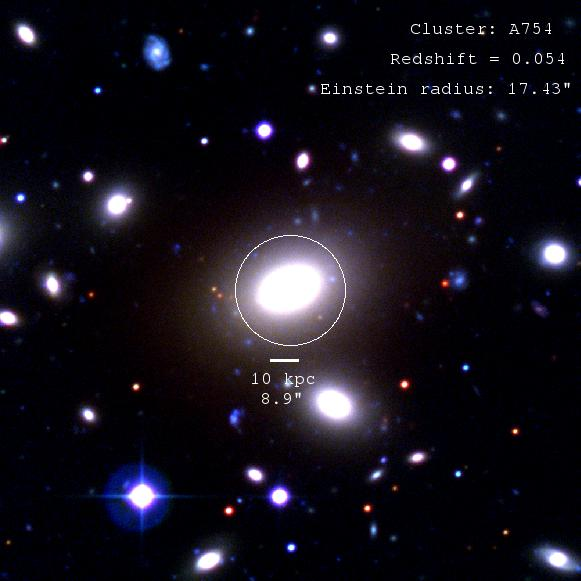
\includegraphics[width=12cm]{images/cA754.jpg}
\caption[M]{G}
\end{figure}

\begin{figure}[H]
\centering
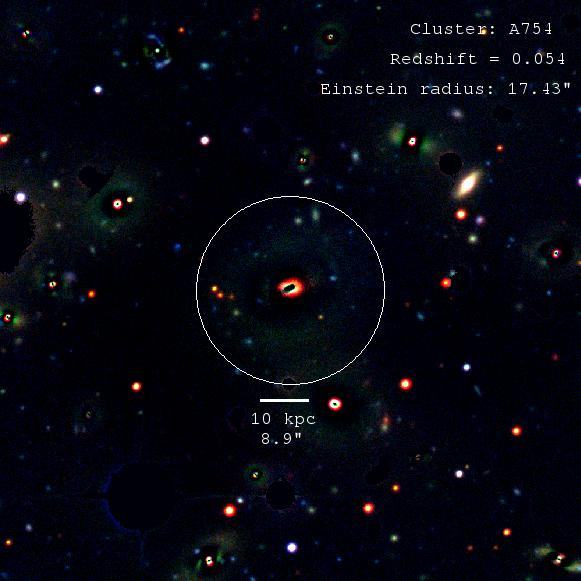
\includegraphics[width=12cm]{images/cA754_galfit.jpg}
\caption[M]{G}
\end{figure}


\section{Photometric Redshift}

(using as reference Benitez, Narciso 2000)